\paragraph{} As we change the problem from a finite and known number of processes with at most one BCA to an unknown number of processes with no restriction on the number of BCA, it is important to look for what is likely to change. Therefore we implemented a DAG random generator (see section~\ref{sec:daggen}) in order to test the possible number of BCA. 
\paragraph{} At the same time we implemented the same algorithm that the one used on a finite and known number of process, except that we now assume that each node $a$ of the DAG contains a hash $h(a)$ of size $k$. We label every node $a$ of the tree with a vector $v(a)$ corresponding to a BF of the predecessors, hence $v(a)_i=\sum_{b\in \mathrm{ancestor}(a)} h(b)_i$, with this labeling we test wether the proposition \ref{propmin} can still be used in some way. From the definition of the labeling we have a weaker version of proposition \ref{propmin} and we wanted to experiment wether we could use it or not.
\begin{proposition}
 If $c$ is a biggest common ancestor of $a$ and $b$ then $v(c) \preccurlyeq \mathrm{min}(v(a),v(b))$. \label{propinf}
\end{proposition}
In our DAG algorithm nodes are placed in different layers, each layer having links only with the previous and the next one. An important parameter to consider is the probability for a node that a node from the previous layer is one of its parents. Examples of the influence of this parameter (called $p$) can be found in section~\ref{sec:daggen}. The "height" of a DAG is the length of the biggest path between two nodes of the DAG. The next graphs show the influence of $p$ and the high of the DAG on the number of BCA and on the number of element verifying the proposition \ref{propinf}.
\begin{figure}[H]
  \centering
 \begin{subfigure}[b]{0.49 \textwidth}
  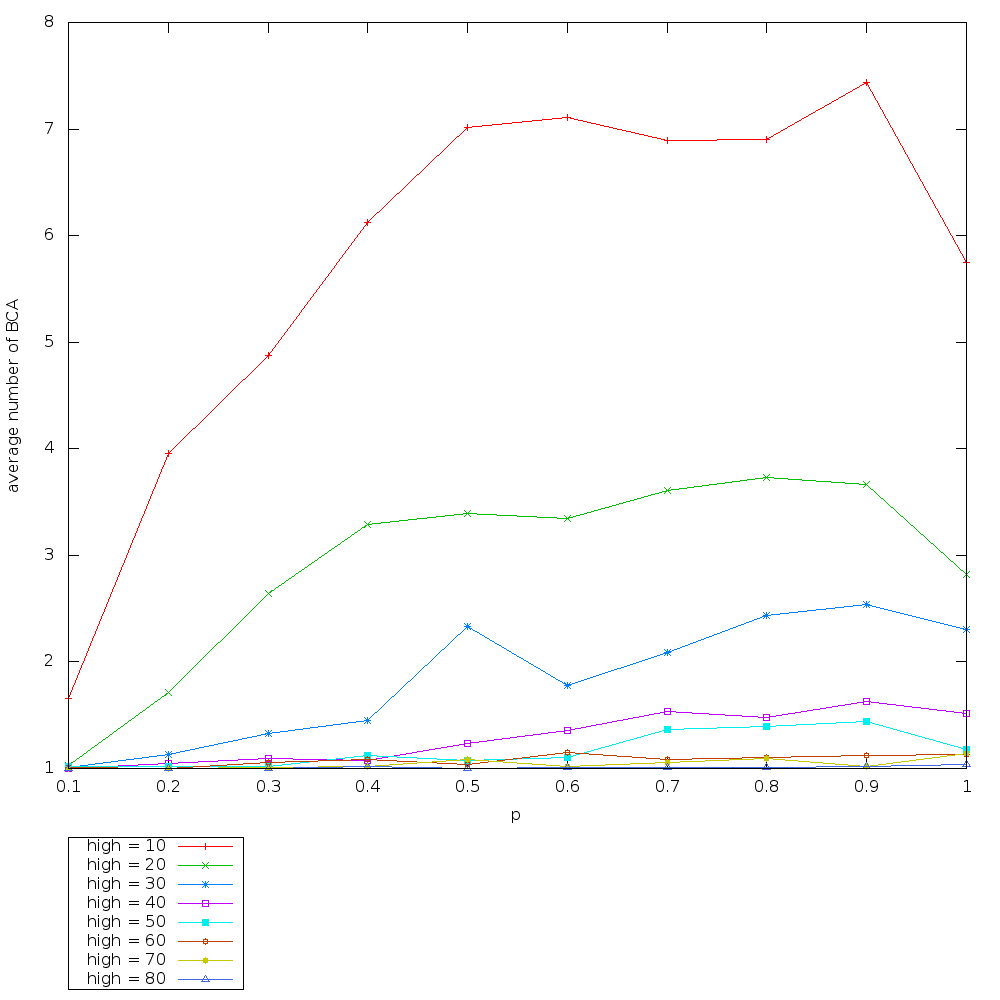
\includegraphics[width = \textwidth]{./image/resultprelim/averagenbbca.png}
  \caption{Number of Biggest Common Ancestor in a DAG with 100 nodes} \label{fig:nbbca}
 \end{subfigure}
 \begin{subfigure}[b]{0.49 \textwidth}
  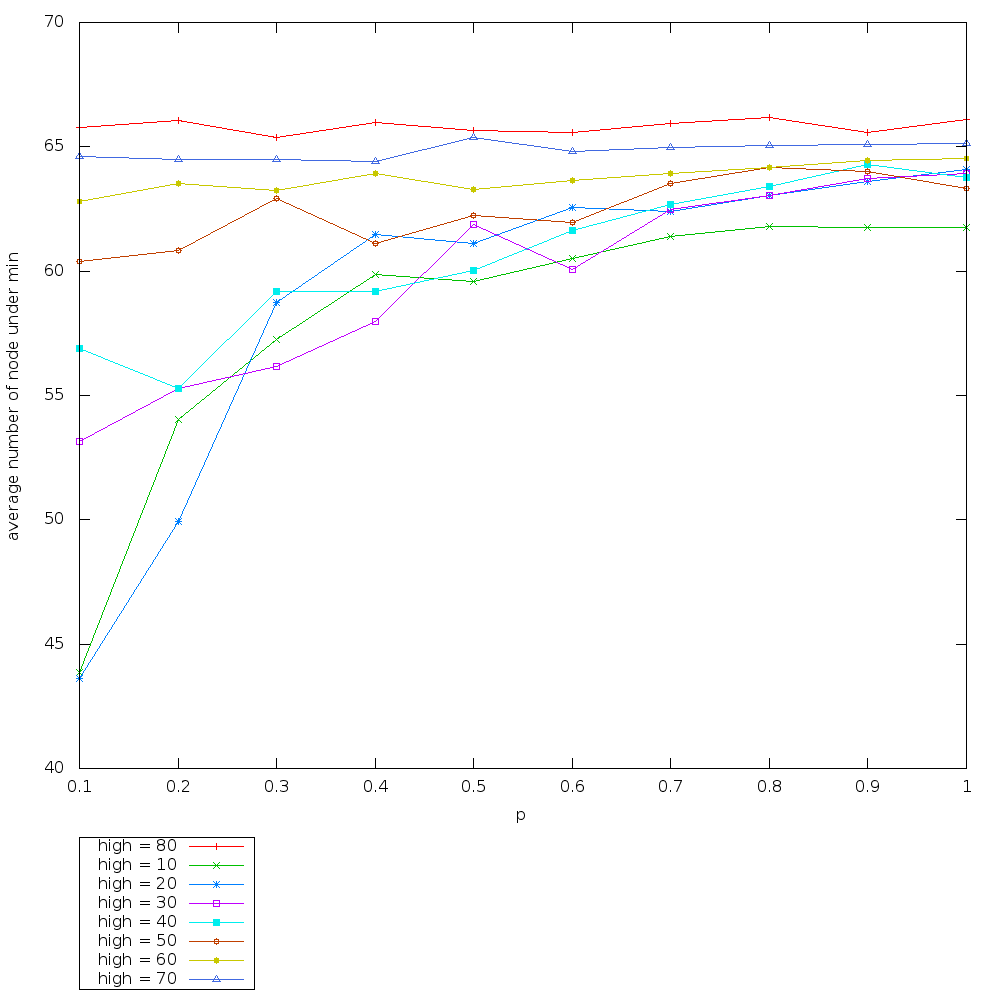
\includegraphics[width = \textwidth]{./image/resultprelim/averagenum.png}
  \caption{Given $a$ and $b$, representation of the number of nodes $c$ verifying $v(c) \preccurlyeq \mathrm{min}(v(a),v(b))$} \label{fig:num}
 \end{subfigure}
 \caption{}
\end{figure}

Figure~\ref{fig:nbbca} shows that the average number of BCA is $2$, this underlines that the assumption on the number of biggest common ancestors was too strong and that we can not rely on the case where there is only one BCA. Figure~\ref{fig:num} shows that the inequality $v(c) \preccurlyeq \mathrm{min}(v(a),v(b))$ holds (in average) for $\frac{1}{3}$ of the nodes, hence adapting the algorithm from the case where we only have a finite and known number of processes might not be a good idea, indeed we reduce the search of the biggest comman ancestor to $\frac{1}{3}$ of the DAG, but the size of the area to search remains linear in the size of the complete DAG.
